\documentclass[times]{ettauth}
%\documentclass[times,doublespace]{ettauth}%For paper submission

\usepackage{acronym}
\usepackage{flafter}
\usepackage{listings}
\usepackage{xcolor}
\usepackage{multirow}
\usepackage{url}

\colorlet{punct}{red!60!black}
\definecolor{background}{HTML}{EEEEEE}
\definecolor{delim}{RGB}{20,105,176}
\colorlet{numb}{magenta!60!black}

\lstdefinelanguage{json}{
    basicstyle=\normalfont\ttfamily,
    numbers=left,
    numberstyle=\scriptsize,
    stepnumber=1,
    numbersep=8pt,
    showstringspaces=false,
    breaklines=true,
    frame=lines,
    backgroundcolor=\color{background},
    literate=
     *{0}{{{\color{numb}0}}}{1}
      {1}{{{\color{numb}1}}}{1}
      {2}{{{\color{numb}2}}}{1}
      {3}{{{\color{numb}3}}}{1}
      {4}{{{\color{numb}4}}}{1}
      {5}{{{\color{numb}5}}}{1}
      {6}{{{\color{numb}6}}}{1}
      {7}{{{\color{numb}7}}}{1}
      {8}{{{\color{numb}8}}}{1}
      {9}{{{\color{numb}9}}}{1}
      {:}{{{\color{punct}{:}}}}{1}
      {,}{{{\color{punct}{,}}}}{1}
      {\{}{{{\color{delim}{\{}}}}{1}
      {\}}{{{\color{delim}{\}}}}}{1}
      {[}{{{\color{delim}{[}}}}{1}
      {]}{{{\color{delim}{]}}}}{1},
}

\newcommand{\specialcell}[2][c]{%
  \begin{tabular}[#1]{@{}c@{}}#2\end{tabular}}

\begin{document}
\newacro{gdp}[GDP]{Gross Domestic Product}
\newacro{citysdk}[CitySDK]{Smart City Service Development Kit and its application Pilots}
\newacro{W3C}[W3C]{World Wide Web Consortium}
\newacro{POI}[POI]{Point of Interest}
\newacro{XML}[XML]{Extensible Markup Language}
\newacro{JSON}[JSON]{JavaScript Object Notation}
\newacro{REST}[REST]{Representational State Transfer}
\newacro{HATEOAS}[HATEOAS]{Hypermedia as the Engine of Application State}
\newacro{poi}[POI]{Point of Interest}
\newacro{gis}[GIS]{Geographical Information System}
\newacro{wg}[WG]{Working Group}
\newacro{iptc}[IPTC]{International Press Telecommunications Council}
\newacro{POIs}[POIs]{Points of Interest}



\runningheads{P. Cruz \emph{et al}}{CitySDK Tourism API - Building value around open data}

\articletype{Special Issue - Smart Cities}

\title{CitySDK Tourism API - Building value around open data}
\author{Pedro Cruz\affil{1},
Ricardo Lopes Pereira\affil{2}\textsuperscript{,}\affil{1}\corrauth\,
Andr\'e Oliveira\affil{3} and 
Geert Monsieur\affil{4}}
\address{
 \affilnum{1}Instituto Superior T\'ecnico, Avenida Rovisco Pais 1, 1049-001 Lisboa, Portugal\\
 \affilnum{2}INESC-ID, Av. Prof. Dr. Cavaco Silva, 2744-016 Porto Salvo, Portugal\\
 \affilnum{3}ISA - Intelligent Sensing Anywhere S.A, Rua D. Manuel I, 30, 3030-320 Coimbra, Portugal\\
 \affilnum{4}European Research Institute in Service Science (ERISS), Tilburg University, Warandelaan 2, 5037AB Tilburg, The Netherlands
}
\corraddr{E-mail: ricardo.pereira@inesc-id.pt}

\begin{abstract}
Tourism is a major social and cultural activity with relevant economic impact.
In an effort to promote their attractions with tourists, some cities have adopted the open-data model, publishing data for programmers to use in their own applications.
Unfortunately each city does it in its own way.

A common API for accessing this data would enable applications to use data from several cities, increasing their potential market while reducing the development costs.
This would benefit developers, cities, which benefit from increased exposure, and tourists, who benefit from better and cheaper applications due to competition.

This article presents the CitySDK Tourism API, which aims to provide access to information about Points of Interest, events and itineraries.
%The API is based on the data model proposed by the W3C POI WG.
It was designed in order to be used by municipalities, regional or national governments as well as other public or private entities interested in publishing touristic information.
The API comprehends a delegation model which enables one server to guide an application towards other servers which have more detailed information, effectively allowing applications to access worldwide information by only knowing a single API endpoint.

The API was created in the context of the CitySDK project, through which a server reference implementation, client libraries and a set of demonstration applications have also been made available, in order to facilitate adoption by cities and application developers.

\end{abstract}

\maketitle

\acresetall
\section{Introduction}

\subsection{Motivation}
\label{s:motivation}
Tourism is a very important social, cultural and economic activity.
According to the World Tourism Organization, in 2012 tourism was responsible for 9\% of the world's \ac{gdp} and for 1 in every 11 jobs.
Tourism generated over 1.3 trillion US\$ in exports and 6\% of the world trade.
2012 was the year where the number of international tourists crossed the 1 billion mark\footnote{\url{http://media.unwto.org/sites/all/files/images/unwto1billioninfographic2.jpg} accessed June 17$^th$, 2013}.
More than half of international tourists elect Europe as their destination~\cite{unwto}.

As vacation time is limited and tourism is a costly activity, tourists wish to make the most of their stay.
There is an industry around travel guides, maps and advice.
This business is also being explored on the Internet and now is making the crossing to the ubiquitous smartphone.
The lower cost of entry when compared to traditional publishing should foster innovation, harvesting the opportunities brought forward by interactivity, positioning systems, wireless Internet access, augmented reality, social networks and crowd-sourcing. 
However, often the foundation for tourism applications is still quality, accurate, reliable information from authoritative sources.

National, regional and city authorities compile large amounts of information to use in their internal processes.
Municipalities understand the value of these data and many have gone through a multi-step process for sharing these data with tourists in order to improve their experience and attract them to the city.
First municipalities created applications (web or mobile) for sharing data with the tourists.
This approach is costly and unsuitable for most cities: the number of visitors is not large enough to recuperate the investment; municipalities are not software houses being unable to keep up with the pace of innovation. 
Furthermore, municipalities are limited in the types of applications they can provide: e.g. publishing negative opinions written by users about an attraction could expose them to liability.

Making data available to third parties is often a better investment and many entities have followed the open-data path.
With access to data, programmers bear the costs and risk, but are free to integrate data from several sources to create novel applications.
Market forces should drive innovation, creating the applications tourists want.
By publishing data openly, municipalities may also aid in the creation of local businesses exploiting this data~\cite{6525605}.
Municipalities may still be forced to publish some applications on their own, should they deem them necessary, but the market not believe them lucrative. 
Still, the open-data model is not without flaws as each entity publishes different datasets using different data formats.
Applications will be restricted to the cities which provide the data required for that application.
Furthermore, programmers are forced to invest into dealing with the particularities of each data representation format, thus limiting the number of data sources which can be included into an application.
These factors will limit the cities covered by applications and thus their potential market, limiting the number and size of the investments.
The local nature of the applications will make them difficult for tourist to find, as they must find the particular application for each city visited.
This problem is also felt for applications created by the municipalities.

The path taken by municipalities has also been traced by other entities related to tourism, such as national and regional governments, museums, concert halls or cultural events organisers.

\subsection{CitySDK}
\label{s:citysdk}

If the same data was made available in the same format by several entities, programmers would be able to reach larger audiences with a smaller investment. 
This would increase competition and tourists would benefit from more applications.
Awareness about the problem exists and efforts are being made to solve the current open-data fragmentation issue.

\ac{citysdk} is an European ICT PSP project involving 29 partners from 9 countries.
The cities of Amsterdam, Barcelona, Helsinki, Istanbul, Lamia, Lisbon, Manchester and Rome are involved.
One of the most important goals of \ac{citysdk} is to create an ecosystem in which the work of an application developer is facilitated by having unified and open city interfaces available across different cities in Europe. 
This means that it should be relatively easy for developers to make use of touristic data coming from multiple European cities, because in such an ecosystem data access is open and unified. 
\ac{citysdk} designs and develops three separate APIs: one for participation services (e.g. FixMyStreet), one for mobility data (e.g. public transport data) and one for touristic information. 
 
In this article, we present the third API, referred to as the \emph{CitySDK Tourism API}, and show how it addresses the problems that municipalities and developers face. 
The CitySDK Tourism API enables access to information about \ac{poi}, events and thematic itineraries.
It can be implemented by municipalities (the main focus in the scope of the \ac{citysdk} project) other government levels and other private or public organisations such as museums or concert halls.
Endpoints for the CitySDK Tourism API are being implemented in Amsterdam, Helsinki, Lamia, Lisbon and Rome.

\subsection{Document structure}
\label{s:structure}
This document is organised into six sections.
In the next section an overview of efforts into providing normalised access to city data is provided.
Section \ref{s:tourim-api} details the CitySDK Tourism API.
Section \ref{s:implementation} describes the reference server implementation and the several client libraries which were produced to make the API easier to use.
An evaluation of the API is presented in  Section \ref{s:evaluation}. 
Finally, Section \ref{s:conclusions} presents the conclusions and describes future work.



\section{Related work}
\label{s:related-work}
The need for common data representation or APIs for tourism data was been present for some time.
In this section we present two major efforts in this field:  EventsML-G2 and \ac{W3C} \ac{POI} \ac{wg}.
We also discuss the Open311 GeoReport API as an example a smartcity API which has successfully been implemented across several cities.

\subsection{EventsML-G2}
EventsML-G2 is a standard for collecting and distributing structured event information, aimed at conveying event information in a news industry environment~\cite{eventsml}. 
This standard is a member of the family of the \ac{iptc} G2-Standards, built on a structural and function framework called the \ac{iptc} News Architecture (NAR), and shares many of its components with the other standards of this family. 
Additionally, the EventsML-G2 makes use of well known industry standards, since its syntax is build on W3C's XML Schema and fully complies with the basic notion of the Semantic Web, the Resource Description Framework (RDF).

One of the main features of the EventsML-G2 standard is it ability to transmit information (facts) about a specific event.
Its comprehensiveness and extensibility makes the standard suitable for covering a big magnitude of event types and cover multiple information facts about a specific event either by literal text (free text) or by codes from specified vocabularies. 

Event though EventsML-G2 can convey information about a \ac{poi} where an event takes place, that is not its focus.
Also, as it strives to represent all types of events, EventsML-G2 is a complex standard, making it difficult to implement and use.

\subsection{\acs{W3C} \acl{POI} \acs{wg}}
\label{section:poi-wg}
The \ac{W3C} is an international community where member organizations, a full-time staff, and the public work together to develop Web standards. 
This community is led by Web inventor Tim Berners-Lee and CEO Jeffrey Jaffe. 

One of its \acp{wg} is the \ac{W3C} \ac{POI} and its mission is to develop technical specifications for the representation of \ac{POI} information on the Web~\cite{w3c-poi}. 
Its Core Recommendation draft defines a generic, flexible, lightweight and extensible \ac{POI} data model, and one normative syntax for the data model based on \acf{XML}.
Although \ac{XML} is the primary model for this specification, other formats are also possible, such as \acf{JSON}.

The data model is shown in Figure~\ref{fig:data-model}~\cite{w3c-poi}.
A brief explanation is given next.

\begin{figure*}
\centering
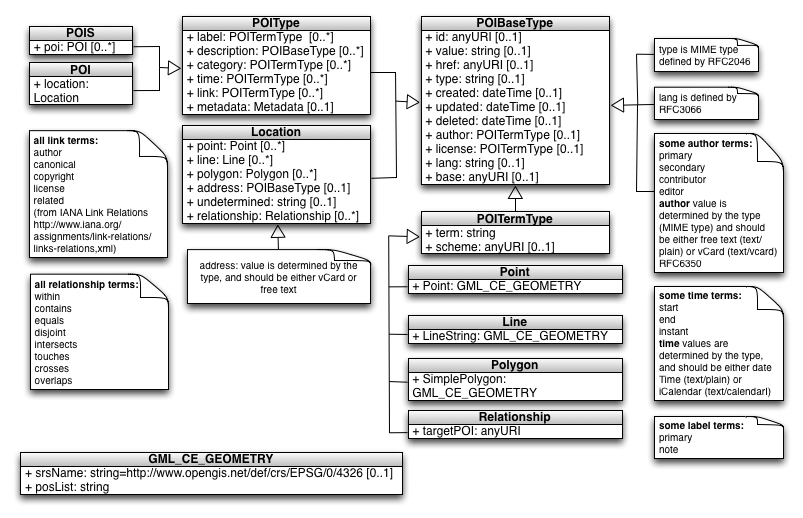
\includegraphics[width=0.9\textwidth]{images/uml}
\caption{W3C POI Core Data Model}
\label{fig:data-model}
\end{figure*}

The data model comprises six entities:
\begin{itemize}
\item \textbf{POIBaseType} is the common entity from which the majority of \ac{POI} entities are derived.
It provides basic properties related with its authorship, licensing, modification dates and identification allowing each element to carry distinct information;
\item \textbf{POITermType} is an abstract entity derived from POIBaseType and adds properties for the management of categorical descriptions (such as the ones seen in category), link, label, author, license and time properties of POIType;
\item \textbf{POIType} is an abstract entity derived from POIBaseType and adds entities for describing, labeling, categorizing and indicating the time span of a \ac{POI} or group of \acp{POI}.
This entity also incudes linking elements to other POIs, external web resources or metadata;
\item \textbf{Location} is an entity that inherits from POIBaseType and provides a flexible description of the location of a \ac{POI}.
A Location can be represented using geodetic coordinates for the center of the POI, line, polygon, civic address, undetermined (representing unresolved locations) or bounding box (relationship element);
\item \textbf{POI} inherits from POIType and adds the Location entity for describing the location of the \ac{POI};
\item Finally, \textbf{POIS} also derives from POIType and can have one or more children entities of type \ac{POI}.
\end{itemize}

This model is flexible and extensible enough to be used within \ac{citysdk} Tourism API to model the various types of data (\ac{poi}, events and thematic itineraries) required.
Its use is described in section~\ref{section:w3cpoi}.

\subsection{Open311 GeoReport API}
The Open311 GeoReport API~\cite{open311} is a standard that is quite popular among cities in the United States of America.
The API allows to both view and report issues which government entities like cities are responsible for addressing.
Traditionally, such issues have been handled by custom web forms or phone based call centers (sometimes using the 311 phone number or other short-code).
The Open311 GeoReport API is designed to allow both government and third party developers to create new applications for submitting and viewing the reports.
The current specification is focused on location-based non-emergency issues such as graffiti, potholes, and street cleaning.

The API is a RESTful API over HTTP that supports both XML and JSON.
It consists of two main kinds of resources: \emph{services} (i.e. things that a municipality can offer to a citizen) and \emph{service requests} (i.e. an issue reported by a citizen).
The methods that are included in the API support a sequence of interactions where a person first sees a list of available service types, selects one and creates a new service request, and then is able to track the status of that and other requests.
However, each method can be accessed independently and some applications may only be focused on querying existing service requests to do analytics.
Similarly, the \ac{citysdk} Tourism API supports different kind of interactions (e.g. listing routes, listing the \acp{poi} of a route, retrieving a \ac{poi}, etc.).


\section{CitySDK Tourism API}
\label{s:tourim-api}
In this section, we will describe some of the key features of the CitySDK Tourism API. We will describe the message format model, how the API is designed and some features that came along with it.

In order to address the challenges presented in Section \ref{s:challenges} and the broader goals of CitySDK (see Section \ref{s:citysdk}) a sound methodology is of critical importance to avoid the pitfalls of deploying an uncontrolled maze of APIs \cite{papazoglou2007,monsieur2012}. The well-adopted service oriented architecture (SOA) development lifecycle (SDLC) \cite{papazoglou2007} provides a solid foundation for service enablement in an orderly fashion so that services can be efficiently used in SOA-based smart city applications. The methodology is based on continuous refinement using a closed loop approach that facilitates designing SOA solutions (e.g. European smart city app) as assemblies of services in which each service assembly is a managed first class aspect of the solution, and, hence, amenable to analysis and change. Developers can then view an smart city app(lication) as a choreographed set of service interactions.

SDLC relies on three fundamental SOA design principles: coupling, cohesion and granularity. These design principles need to guarantee that services are self-contained and come equipped with clearly defined boundaries and interfaces to allow for service composability. Standards and reference models (e.g. W3C POI) are crucial in coping with such design principles. Typically, these standards improve SOA design by defining (sector-specific) business concepts that have an high-degree of cohesion and low-degree of coupling. The design of the tourism API is fundamentally based on W3C POI (see Section \ref{section:w3cpoi}). By reusing existing standards such as W3C POI the chance for adoption is substantially increased. Furthermore, it reduces coupling because developers are not bound to use message formats linked to a specific service implementation \cite{papazoglou2007}.

Before diving into a deeper description of the CitySDK API there are three fundamental aspects that should be mentioned. The API provides the following: four types of data models, methods to retrieve information concerning these same data models and also, methods and description fields that retrieve the relationships between each of them. Regarding the data models we provide the following:
\begin{itemize}
\item \textbf{\ac{POI}} describes various places in a given city, ranging from monuments and museums to eating places and cultural venues; 
\item \textbf{Event} describes cultural events that happened or are about to happen in the city;
\item \textbf{Itineraries} describe a group of \acp{POI} organized in such a way that they form an itinerary of a given topic, e.g., the life of a given person, the history of a given region or even just specific sightseeing spots;
\item \textbf{Categories/Tags} describe a list of available categories and tagging terms for each of the aforementioned models.
\end{itemize}

Each model can also be grouped into a list of its own type, that is, each data model has a listing model where each element is either a \ac{POI}, Event, Itinerary or a Category/Tag.

We now present the key features of the API.

\subsection{W3C POI Model in the API}
\label{section:w3cpoi}
As mentioned before, our API provides four data models: Points of Interest, Events, Itineraries and Categorization data. These models are mapped using the W3C POI Model presented in section~\ref{section:poi-wg}. We will now present how we modelled each data type.

The \textbf{\acf{POI}} are the most easily modelled element of the API. Since the W3C POI Model is specific for this type of data we used its already specified properties to map our data model. So, the Points of Interest are mapped and described by using the \textit{POI} entities directly. It should be mentioned that, since the \ac{POI} is somewhat very detailed and verbose, we defined two granularities for this element: a minimal description, that only includes the key essential properties and a complete model, which is the original W3C POI Data Model. The minimal model is used to map each element of a list of \ac{POI}. Such list is described by the \textit{POIS} entity, but it does not use the descriptive properties of \textit{POIType}.

The \textbf{Events} are modelled the same way the \acp{POI} were, but instead of having a \textit{Location} entity completly specified, we used the \textit{relationship} property of the same entity to relate a given Event to a \ac{POI} and ommited the \textit{address} and \textit{undetermined} properties. So, we have an Event completly described using the \textit{POI} entity and use the \textit{relationship} property to also specify and descibe the location of the Event. An Events list is modeled using the \textit{POIS} entity, much like the \acp{POI}, but it does not have a different granularity and the root name is \textit{event} instead of \textit{poi}.

The \textbf{Itineraries} is somewhat more complex. It is defined by using the \textit{POIS} entity and all of its descriptive properties. So, we have the description of the Itinerary itself by using the \textit{POIType} descriptive properties and have the group of \acp{POI} by using the \textit{poi} property named as \textit{pois} (so not to confuse with the mentioned list of \ac{POI}). It should be mentioned that these \acp{POI} are not the original \acp{POI}, but are described in the context of the Itinerary, though they include the relationship with its original counterpart, so to fetch the actual description. Finally and like the previous two, the Itineraries has a list associated with it. Much like the \ac{POI}, it has a second granularity - a minimal version - in which only the description of each Itinerary is included and their \acp{POI} are ommited.

The \textbf{Categories/Tags} are equal in nature, but a Category provides a recursive format that the Tags do not. Both borrow from the W3C POI Data Model, but their format is more specific to the needs of the API, rather than following the mentioned model. So, a Category simply follows the \textit{POIType} entity and allows recursiveness and a Tag borrows its properties from the \textit{POIBaseType} to specify a language and value.

At last, most of the terms used in the POITermType are the suggestions made by the working group itself. However, we've added three more terms regarding price, waiting time, occupation and accessibility information for handicapped people. Such terms are identified as X-citysdk/price, X-citysdk/waiting-time, X-citysdk/occupation and X-citysdk/accessibility-textual and X-citysdk/accessibility-properties, respectively.

The presented models are used in the message format of the API, in the format of \ac{JSON} (like we have seen previously).

\subsection{API Description}
\label{s:api-description}
The API follows the \ac{REST} architectural design~\cite{Fielding:2002:PDM:514183.514185}. Thus, we designed a RESTful API over HTTP using JSON. Hence, for each of the presented models we designed various methods to obtain certain data following certain parameters. Many of the parameters are common between the \acp{POI}, Events and Itineraries, such as the ability to search for each one of them using a categorical reference, a description or using coordinates. Also, we have provided limitation parameters to allow applications to lazy load the data presented by the API. Of course, there are some parameters that are specific to the data model, e.g., if we search using a description of the \acp{POI}, one can ask for either the minimal or complete version or in the case of the Events, we can search using time spans. Furthermore, and for both \acp{POI} and Events, one can also search for the relation of a single \ac{POI}/Event with other \acp{POI}/Events. One final method is the ability to search using QR Code or Barcodes. Using a single method and providing the textual or bar code information, we retrieve any POIs, Events or Itinerary that match such information.

As for the categorization models, we have provided methods to retrieve the categorical information for each of the aforementioned models by using a list parameter indicating which type of data we wish to retrieve. Such results can also be limited by using the same limitation parameters mentioned above.

Another feature of the API, and somewhat ignored by many REST systems, is complying to the \acf{HATEOAS} constraint of Fielding's dissertation. This constraint states that a client interacts with a network application entirely through hypermedia provided dynamically by the application servers. Therefore, it needs no prior knowledge about how to interact with any particular application or server beyond a generic understanding of hypermedia. We made use of this constraint in three ways:
\begin{enumerate}
\item From the entry URL - the only URL that the client needs to know - we present the resources made available by the visited server;
\item Each of the Data Models has an identification (specified by a base URL and ID) that allows to fetch information about that specific model;
\item The POIs, Events and Itineraries can be further described by using a \textit{described-by} (in the links property) which indicates an entry point to another server, which can provide further data on that specific entity.
\end{enumerate}

The mentioned resources indicate to the client, which models and which parameters are available in a given server. These models can be presented by the key-values found in the response message, e.g., if a \textit{find-poi} key is found, then the server supports \acp{POI}. As for the allowed searching parameters we have used the URI Template RFC~\cite{uri-template}. This way, we allowed a simple yet descriptive manner to indicate which parameters and which data is available and can be fetched.

This feature allowed our system to delegate responsibilities, as we will see in Section~\ref{delegation}.

\subsection{Delegation}
\label{delegation}
As mentioned in Section~\ref{s:api-description} we designed an API based on hypermedia content. Such feature allows the use of delegation between the various entities involved in the system: a world-wide directory containing the endpoints of CitySDK-enabled servers; the city servers providing CitySDK data; and a more granular server provided by museums or any other venues which give more detailed information about that specific \ac{POI}, Event or Itinerary. Figure~\ref{fig:delegation} shows a diagram of the interactions between each entity.

\begin{figure}
\centering
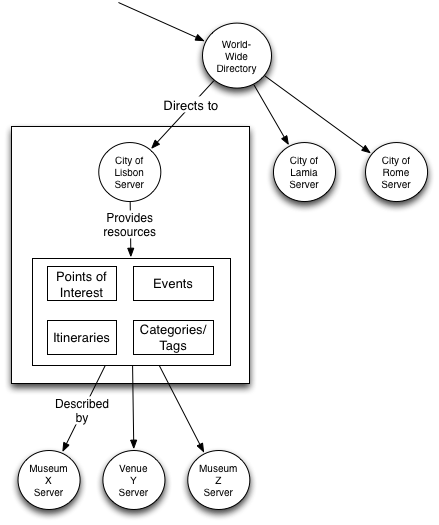
\includegraphics[width=0.4\textwidth]{images/delegation}
\caption{Delegation Model}
\label{fig:delegation}
\end{figure}

Further explaining the diagram, a client visits the world-wide directory and provides a given geodetic coordinates and an API key. The world-wide directory then directs the client based on the provided set of  coordinates and on the validation of the API key.

The client then visits the provided server address, in which the resources are provided, ending by querying the given server for any of the available data. 

At last, the client may further detail the information given by the server by visiting a museum or venue's server. Such server can be known if the provided resource has a \textit{described-by} parameter in the \textit{links} property containing the endpoint URL.

\section{Implementation}
\label{s:implementation}
This section describes the implementation details of the API framework and, in specific, the details of an example real implementation scenario provided for the Lisbon municipality. 

In general terms, the implementation of the platform was planned having in mind key points to ensure its long term sustainability and scalability, adapted not only for the demands expected for the CitySDK project during its development and deployment lifespan but also for its expansion to other cities with different profiles, in terms of expected client demand and provided volume of open-data.

\subsection{Platform Architecture}
Figure \ref{fig:architecture} shows the composing components of the architecture of the implemented CitySDK platform. 

\begin{figure}[!ht]
\centering
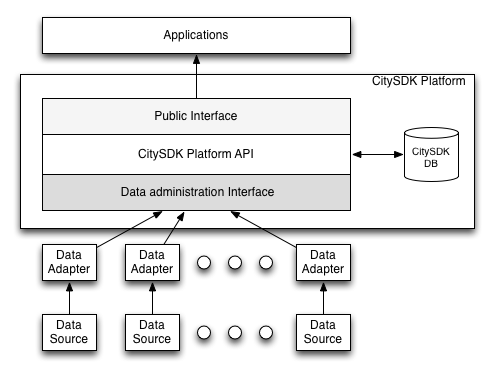
\includegraphics[width=0.4\textwidth]{images/architecture}
\caption{CitySDK platform architecture}
\label{fig:architecture}
\end{figure}

In the platform's architecture, the city acts as a data provider who provides one or more relevant touristic information datasets. CitySDK platform is capable of incorporating several distinct data sources by using a modular approach where each one of the data sources provide their information through a Data Adapter module. 
The Data Adapter module is a component developed to retrieve raw data from a data source in its native format (XML, JSON, CSV or other) using the data source's native access form (web service, file, database or other) and provide the touristic data (regarding \acp{POI}, Events and Itineraries) to be stored in the platform in the data format presented earlier. 
The Data Adapter module interacts with the CitySDK platform by invoking its Authenticated data administration REST API for manipulating (inserting, updating or deleting) data elements. 
The Data Adapter module is not only responsible for inserting data elements in the platform but also for maintaining them by updating or deleting the data elements as needed through the platform's life. 
In most common cases each data source should have its Data Adapter module but it is also possible to foresee a scenario where a single Data Adapter module retrieves from several data sources if they are similar in terms of access and provide data in a similar format. 
Despite of not being the case for the example implementation of the platform in Lisbon municipality scenario neither in the core scope of the CitySDK project's requirements, the platform owner may allow third party data sources (i.e. not controlled by the platform owner such as commercial partners) to insert and maintain data in the platform; the platform is capable of managing several distinct data owners by using its authentication and data ownership mechanism.

Despite of the CitySDK's platform having a single API endpoint, it can be divided in two distinct conceptual APIs: the public API and the data administration API. 
The public API is the API where the client end-user applications (e.g. mobile or web applications) can interact to retrieve the touristic data available in the platform by using the available access and search methods. 
Although not implemented at the time of writing, an enhancement is planned for this public API by providing an access key system, similar to the one found in some third party interned based services (such as Google Maps), enabling keys to be provided to application developers for use in their applications to access the platform. 
The intent of this access key system is not to restrict access to the CitySDK platform (as a non-keyed access will be always available with limited/lower quality of service) but to prevent abuse and at the same time provide some feedback to the platform owners on the used client applications. 
The second API, the data administration API, requiring a valid authentication to access it, is the interface to be used for the purpose of manipulating data elements (\ac{POI}, Events, Itineraries and their respective categorical information) in the platform. 
This data administration interface is used by the Data Adapter modules to maintain their data in the platform, enabling the operations of inserting new data elements, update or deletion of the existing elements in the platform. 
All the data elements operated through the data administration API are verified against a set of rules and constraints needed to maintain the sanity of the platform and its data.

The CitySDK platform maintains data retrieved in its own database. 
As the platform must be capable of serving a high number of requests per interval of time, special care was taken when choosing and designing the platform's database. 
In order to optimize the API and database load and increase the potential platform's throughput, data stored in the database is in a format similar to the W3C POI format (with some minor needed variations), almost ready for being served promptly to the requesting clients, requiring the minimal processing effort as possible in both the platform's database (in terms of number of queries and query complexity) and platform's API engine (in terms of needed processing effort to build the response to the clients).

\subsection{Implementation details}
As shown in the architecture representation (Figure~\ref{fig:architecture}), the core of the CitySDK platform is based on a main component, the application service denoted as "CitySDK Platform API" in the figure, as it provides the previously mentioned APIs (public and data administration), and is aided by a platform's database. 

The CitySDK application service was implemented taking in account the CitySDK platform's requirements in terms of providing a REST interface and having high information throughput capability to serve its end-user clients. 
The application service was implemented using as base a fast and lightweight open-source REST Web Services framework named ServicStack\footnote{\url{http://www.servicestack.net/}}. The ServiceStack base framework is responsible for handling the protocol part of the CitySDK's platform interface, converting the received web requests into simple method calls and converting back the method return values into a web response. 
Despite of being possible to run the ServiceStack base framework in a Mono\footnote{\url{http://www.mono-project.com/Main_Page}} making a Linux based environment a possible hosting solution for the CitySDK platform, for the Lisbon's platform instance a Windows\footnote{Microsoft Windows Server 2012} based environment in conjunction with the Microsoft .Net framework solution was used and remains the recommended platform while no extensive testing was performed on the platform using the alternative Linux/Mongo solution.

For the CitySDK platform's database, an open-source high performance document database named mongoDB\footnote{\url{http://www.mongodb.org/}} was used instead of the traditional relational SQL based database. 
The choice of this database was mainly related with the high performance for the foreseen database request types. 
This document database is the CitySDK platform data backend and stores both the platform's data models and some minor administrative data (e.g. access credentials). 
The data models are stored in an optimal format, taking advantage of the characteristics inherited from the fact that the database in use is a document database, aiming to require the minimal effort for the platform's engine to adapt the retrieved data elements to the replies for the clients requests. 
Although the used database is not a relational database, it gives also the possibility to index any of the stored document's attributes to enable the possibility of performing quicker indexed searches. 
The database also has the desired capabilities of a \ac{gis} enabled database such as PostGIS\footnote{\url{http://postgis.net/}}, enabling the possibility to perform geographical queries to the data such as the ones required to search for a data element within a specified polygon or within a distance from a specified point in the city. 
The flexibility of the stored data structure is also a valued property of the database, enabling the possibility to have stored objects with different characteristics, as permitted by the W3C POI model used in the CitySDK.

Although Data Adapter modules are not part of the CitySDK platform's itself, they are essential for the its life and perform the important task of populating it with valuable data. 
These modules have to be CitySDK-compliant on the data output side and datasource-compliant on the data input side, transforming the datasource's data from its native format into the W3C POI format liable to be inserted into the platform. 
For the case of the Lisbon implementation, a single database containing aggregated data from \acp{POI} and Events (including the relation of the \ac{POI} where Events occur whenever possible) was identified, so only a Data Adapter module was needed to be implemented for the two types of data. 
The implemented module runs as a service and, as the volatility of the data is very low (at maximum few records are updated during a day), the data updating process runs once a day during the empty hours. 
The data updating process consists on inserting the new data elements found on the city's database on the CitySDK platform, update any change perceived on the city's database to the CitySDK platform and cleaning up the deleted data elements from the CitySDK platform. 
Regarding Itineraries, Lisbon municipality provides three distinct static elements (no update is made to them) and publishes them manually to be inserted in the CitySDK platform on the form of text files; these text files are imported to the platform using a Data Adapter that runs once as a stand-alone module. 
In future, when Lisbon municipality computerizes the Itineraries data, the Data adapter can be converted to a service similar to the one used for importation of \ac{POI} and Events which automatically imports/updates the data elements.

\subsection{Client-side stubs}
As a final mention for the implementation details we present our client stubs. 

To facilitade the development cycles of potential developers, we provided four libraries which abstract the use of the API and parsing of the received data. These libraries are very similar in usage as they provide equal naming conventions for methods to perform requests, as well, as to read any of the received data.

The libraries are written in Java, JavaScript/jQuery, PHP and Objective-C and are available online as well as their corresponding documentation and usage examples. They can be found through the project's website~\footnote{\url{http://www.citysdk.eu/developers/}}.

\section{Evaluation}
\label{s:evaluation}

\subsection{Compliance to the CitySDK performance requirements}
CitySDK project established a performance requirement in terms of minimum number of requests per second that the platform should be able to serve, calculated from the indicators in terms of expected public adherence to the CitySDK platform at the end of the project timespan through the applications to be developed by 3rd party developers. 
The calculated number was 105 requests per second. 
In order to assure that the performance requirement of the CitySDK was fulfiled, a simple test using 150 distinct requests for \acp{POI} was performed against a CitySDK platform loaded with a database populated with real data from Lisbon municipality containing around 3800 independent \acp{POI}. 
The tool used to perform the test was Siege\footnote{\url{http://www.joedog.org/siege-home/}} version 2.70 and the testing server was running in a Microsoft Windows 7 64bit powered by a Intel i5 processor at 2.9GHz with 8GB of RAM memory.
A batch of 5 tests composed by 10.000 repetitions of 150 independent \acp{POI} requests was performed resulting on the final average capacity of 620 request per second which proved that the implemented CitySDK platform was fully compliant with the required performance capacity.

\subsection{Proof of Concept Applications}
To further test our client libraries and API, we developed a group of key applications in various programming languages and frameworks.
The first application made use of the Java library. 
We developed an Android application which displays \acp{POI}, Events and Itineraries following a user's criteria, e.g using categorical information and/or using coordinates. 
It displays the retrieved data in both list and map format (in the case of the Itineraries, it would draw the route itself). 
Its main goal is to use the API to its fullest and demonstrate the various possibilities for applications.

We've also developed a set of applications making use of the JavaScript/jQuery library. These set of applications are an Event's calendar, and thus it makes specific use of Events and time/categories-related searches and a Map displaying all types of data models.

At last, we developed a Augmented Reality application using the Layar framework by developing a PHP web-server and thus, in this case, we used the PHP library. 
This application simply makes use of the position, camera and sensors of the user's device to display information about the surroundings and/or the building being displayed in the screen.

The Objective-C library was not ignored, since an application is being developed at the moment.

% talk about the benefits of the API. new business models etc.
% companies which run directories for small bussiness to provide detailed info
% benefits and exemples of delegation
% museum capacity and queue lenght
% disabled info


\section{Conclusions}
\label{s:conclusions}
This article presents the \ac{citysdk} Tourism API, which is based on the data model defined by the \ac{w3c} \ac{poi} \ac{wg}.
This API provides access to information about \ac{POI}, events and itineraries, enabling municipalities, regional or national governments as well as other public or private entities to publish touristic information for developers to incorporate into their applications.
This open-data model is expected to increase the market for tourism applications while lowering the cost of entry.
The increased competition should drive down application costs while increasing their quality, benefiting tourists.
Data publishers also benefit from increased exposure, increasing the appeal and visibility of their attractions.

Besides the API definition, a reference server implementation and client libraries for the most popular programming languages have been made available in the context of the \ac{citysdk} project.
This will facilitate the adoption of \ac{citysdk} Tourism API outside the project.

In the future, we intend to follow the implementation of the \ac{citysdk} Tourism API in several cities and refine the API as new challenges arise.
In the near future we intend to develop processes for facilitating the management of a worldwide directory for \ac{citysdk} Tourism API endpoints, enabling new cities to easily joint this service.
A single endpoint is crucial for enabling existing applications to take advantage of new \ac{citysdk} Tourism API deployments as they become available.

Developer keys are often used to identify developers, providing a way for server owners to throttle API usage in order to deter heavy-hitters and providing an incentive for programmers to produce efficient code.
These can also be used to ban misbehaving applications from using an API.
A worldwide directory would only make sense if developer keys are portable among different endpoints.
Currently we are working on a model for distributed developer keys issuing which does not compromise these goals.


\acks
The \ac{citysdk} project is financed by the European Commission under the Information and Communication Technologies Policy Support Programme (ICT PSP) as part of the Competitiveness and Innovation framework Programme (CIP).

This work was partially supported by national funds through FCT – Funda\c c\~ao para a Ci\^encia e a Tecnologia, under project PEst-OE/EEI/LA0021/2013

\bibliographystyle{wileyj}
\bibliography{references}

\end{document}


% Local IspellDict: "british"
% Local IspellPersDict: "~~/.ispell-English"

% Local Variables:
% mode: flyspell
% End:
